\documentclass[french, output=paper]{langscibook}
\ChapterDOI{10.5281/zenodo.10280608}

\author{Maria Kihlstedt\orcid{}\affiliation{Université de Paris-Nanterre}}

\title[Passé composé/imparfait chez des enfants bilingues français-suédois]
      {Développement du passé composé\slash imparfait et variation des tâches chez quelques enfants bilingues français-suédois}

\abstract{Plusieurs études ont exploré l’acquisition du temps et de l’aspect en français langue première (\citealt{Sabeau-Jouannet1977, Schlyter1990, Labelle1994, Jakubowicz2003, Meisel2009}) et en français langue seconde (\citealt{DietrichEtAl1995, Véronique1995le, Kihlstedt2002, Ayoun2004, Granget2004, Howard2005, Izquierdo2009, McManus2013, Véronique2014Description}) avec une variété des L1. En revanche les études qui comparent l’acquisition bilingue initiale dit simultanée ou successive sont plus rares. Dans cette étude qualitative, deux enfants qui ont commencé leur exposition au français entre l’âge de 3 et 4 ans ont été suivis longitudinalement de 6 à 8 ans. Ils sont comparés à (i) deux enfants bilingues simultanés depuis la naissance et (ii) deux enfants L1 français des mêmes âges, tous issus du corpus du projet franco-suédois STUF. La question de base concerne le développement de l’enfant au bilinguisme successif : se différencie-t-il du développement des enfants issus du bilinguisme simultané et des enfants L1 dans le domaine du temps et de l’aspect du passé ? La question est examinée dans deux tâches différentes (conversations spontanées et un test de morphologie temporelle). Les comparaisons montrent que l’utilisation spontanée des temps verbaux suivrait des étapes communes, avec un léger retard des enfants L2, alors que dans des tests plus ciblés, les bilingues successifs se différencient clairement des deux autres groupes d’enfants. Les résultats sont discutés en fonction de l’âge du début de l’acquisition et de l’influence de la tâche.
\keywords{bilinguisme simultané, bilinguisme successif, morphologie temporelle, temps et aspect, imparfait, AOA (age of onset)}}

\IfFileExists{../localcommands.tex}{
  \addbibresource{../localbibliography.bib}
  % add all extra packages you need to load to this file

\usepackage{tabularx,multicol}
\usepackage{url}
\urlstyle{same}

\usepackage{listings}
\lstset{basicstyle=\ttfamily,tabsize=2,breaklines=true}

\usepackage{langsci-basic}
\usepackage{langsci-optional}
\usepackage{langsci-lgr}
\usepackage{langsci-osl}
% \usepackage{./langsci/styles/langsci-lgr}
% \usepackage{./langsci/styles/langsci-osl}
% \usepackage{langsci-gb4e}

\usepackage{tikz}
\usetikzlibrary{patterns,calc}
\pgfdeclarepatternformonly{south east lines}{\pgfqpoint{-0pt}{-0pt}}{\pgfqpoint{3pt}{3pt}}{\pgfqpoint{3pt}{3pt}}{
    \pgfsetlinewidth{0.6pt}
    \pgfpathmoveto{\pgfqpoint{0pt}{3pt}}
    \pgfpathlineto{\pgfqpoint{3pt}{0pt}}
    \pgfpathmoveto{\pgfqpoint{.2pt}{-.2pt}}
    \pgfpathlineto{\pgfqpoint{-.2pt}{.2pt}}
    \pgfpathmoveto{\pgfqpoint{3.2pt}{2.8pt}}
    \pgfpathlineto{\pgfqpoint{2.8pt}{3.2pt}}
    \pgfusepath{stroke}}
    
\usepackage{stmaryrd}
\usepackage{wasysym}
\usepackage{multirow}
\usepackage{caption}
\usepackage{subcaption}
\usepackage{mathrsfs}
\usepackage{qtree}

\usepackage{linguex}


  %pminos do not split footnotes
% \interfootnotelinepenalty=10000 %Footnote in Laporte chapters has to be split SN


%\DeclareIndexNameFormat{default}{%
%\nameparts{#1}%
%\usebibmacro{index:name}%
%{\index[names]}%
%{\namepartfamily}%
%{\namepartgiveni}%
% {}% L1
% {}% L2
%{\namepartprefix}% generates spurious space L3
%{\namepartsuffix}% generates spurious space L4
%}

%  {\DeclareIndexNameFormat{default}{%
%     \usebibmacro{index:name}{\index[names]}{#1}{#3}{#5}{#7}}}

%\DeclareIndexNameFormat{default}{%
%  \usebibmacro{index:name}{\sindex[nom]}{#1}{#3}{#5}{#7}}

%\DeclareIndexNameFormat{default}{%
%  \usebibmacro{index:name}{\sindex[person]}{#1}{#3}{#5}{#7}}
%\DeclareIndexNameFormat{default}{%
%\nameparts{#1} \usebibmacro{index:name}{\sindex[person]]}{\namepartfamily}{‌​\namepartgiven}{\nam‌​epartprefix}{\namepa‌​rtsuffix}}

%\newcommand{\smiley}{:)}

%\renewbibmacro*{index:name}[5]{%
%\usebibmacro{index:entry}{#1}%
%{\iffieldundef{usera}{}{\thefield{usera}\actualoperator}\mkbibindexname{#2}{#3}{#4}{#5}}}

% \newcommand{\noop}[1]{}

%remove for final
%\overfullrule=1mm

\newcommand{\tobi}[2]}}
\renewcommand{\S}[1]{\tobi{#1}{\textsc{*}}}

% this volume references
% puts: [this volume]
% already defined: \citetv
%\newcommand{\citepv}[1]{(\citeauthor{#1} \citeyear*{#1} [this volume])}
\newcommand{\citealtv}[1]{\citeauthor{#1} \citeyear*{#1} [this volume]}

%parentheses around example number
\newcommand{\pref}[1]{(\ref{#1})}

% in-text examples

\newcommand{\lnex}[1]{\textit{#1}} %target lang word
\newcommand{\lnlit}[1]{(lit.: `#1')} %literal reading
\newcommand{\lnlat}[1]{(#1)} % latinization
\newcommand{\lntrans}[1]{`#1'} %translation
\newcommand{\lnexl}[2]%
{\lnex{#1}{} \lnlat{#2}} % ex with latinization
\newcommand{\lnexlat}[3]{\lnex{#1}{} \lnlat{#2}{} \lntrans{#3}} % ex with latinization and tranl.

%ch01
\newcommand{\co}[1]{\mbox{\textbf{#1}}}

%ch09

\newcommand{\cyrbulg}[1]{\begin{otherlanguage*}{bulgarian}#1\end{otherlanguage*}}


%ch10
\newcommand{\nlp}{{\small NLP}}
\newcommand{\mwe}{{\small MWE}}
\newcommand{\rae}{{\small RAE}}
\newcommand{\lvc}{{\small LVC}}
\newcommand{\pos}{{\small P}o{\small S}}
%\newcommand{\todo}[1]{ \textcolor{red}{#1} }

%\renewcommand{\labelenumi}{\theenumi}
%\ainamefmt{{vv}{ll}{, ff}{, jj}} % fullname

\newcommand{\biberror}[1]{{\color{red}#1}}

\newcommand{\osenovaitem}{--~} 
  %% hyphenation points for line breaks
%% Normally, automatic hyphenation in LaTeX is very good
%% If a word is mis-hyphenated, add it to this file
%%
%% add information to TeX file before \begin{document} with:
%% %% hyphenation points for line breaks
%% Normally, automatic hyphenation in LaTeX is very good
%% If a word is mis-hyphenated, add it to this file
%%
%% add information to TeX file before \begin{document} with:
%% %% hyphenation points for line breaks
%% Normally, automatic hyphenation in LaTeX is very good
%% If a word is mis-hyphenated, add it to this file
%%
%% add information to TeX file before \begin{document} with:
%% \include{localhyphenation}
\hyphenation{
    Beck-man
    Ngu-yen
    back-chan-nel
    back-chan-nels
    mo-not-o-nous
    ste-reo-typ-i-cal
}

\hyphenation{
    Beck-man
    Ngu-yen
    back-chan-nel
    back-chan-nels
    mo-not-o-nous
    ste-reo-typ-i-cal
}

\hyphenation{
    Beck-man
    Ngu-yen
    back-chan-nel
    back-chan-nels
    mo-not-o-nous
    ste-reo-typ-i-cal
}
 
  \togglepaper[2]%%chapternumber
}{}

\begin{document}
\begin{otherlanguage}{french}
\lsFrenchChapterSettings{}
\AffiliationsWithoutIndexing{}
\maketitle 
 

\section{Introduction}\largerpage
Une grande partie des recherches sur le bilinguisme enfantin se penche sur les différences et les similitudes entre enfants monolingues et enfants bilingues \textit{simultanés} (ayant été activement exposés à deux langues depuis la naissance). Ces recherches se consacrent pour la plupart à de très jeunes enfants (1 à 4 ans) et mettent souvent l’accent sur les similitudes entre les deux groupes. L’acquisition initiale bilingue (désormais, \textit{2L1}) ressemblerait à l’acquisition monolingue de chacune des deux langues au niveau des itinéraires  acquisitionnels. En revanche, des différences au niveau du rythme d’acquisition, à savoir un léger retard par rapport aux monolingues, peuvent avoir lieu (\citealt{SchlyterHâkansson1994, Genesee2003, DeHouwer2005}). Plus récemment, un nombre croissant d’études ont commencé à s’intéresser aux enfants issus du bilinguisme \textit{successif} (ayant acquis une première langue, puis une deuxième à un âge précoce, désormais \textit{eL2}), (\citealt{GranfeldtEtAl2007, Paradis2007, Kihlstedt2009, Meisel2009, TracyThoma2009, Schlyter2011, Unsworth2016}). En ce qui concerne l’exposition initiale au français, les deux groupes de bilingues s’opposent. D’une part, les bilingues simultanés grandissent avec deux langues premières. D’autre part, les bilingues successifs entament l’acquisition d’une deuxième langue (dans notre cas, le français) alors que le développement de la première n’est pas encore terminée. Les bilingues successifs se distinguent également des adultes qui acquièrent une langue seconde par le fait que ces derniers possèdent déjà un système cognitif entièrement abouti au début de l’apprentissage, alors qu’il est en cours de développement chez les enfants bilingues. Les similarités entre l’acquisition bilingue successive et l’acquisition bilingue simultanée -- où le système cognitif universel se développe en parallèle avec deux systèmes linguistiques -- n’ont été que très peu explorées. Dans la présente étude, nous comparons le développement de ces deux types de bilinguisme enfantin, en nous focalisant essentiellement sur le bilinguisme successif.

Notre étude s’inscrit dans un projet qui a été mené conjointement à l’université suédoise de Lund et à l’université de Paris-Nanterre, intitulé STUF (\textit{Startâlder och utveckling i franska}, «~Age du début de l’acquisition et développement en français~»). L’intérêt principal de ce projet était de tenter de dégager d’éventuelles différences dans le développement du français lorsque l’acquisition débute à des âges différents. Les données de la présente étude sont issus du corpus STUF. Nos résultats portent sur le développement de la morphologie temporelle du passé chez deux enfants bilingues simultanés, deux enfants bilingues successifs et deux enfants L1, tous suivis de 6 à 8 ans. Dans les études qui se sont penchées sur ce type de comparaisons, les enfants dits \textit{2L1} sont exposés à deux langues dès la naissance, généralement dans une famille avec un parent qui est locuteur natif de la langue qu’il utilise avec son enfant. Les enfants dits \textit{eL2} sont exposés à une langue seconde pendant l’enfance mais débutent l’acquisition de celle-ci plus tardivement que les bilingues simultanés, souvent au cours de la scolarisation. Selon \citet{Meisel2009}, l’acquisition eL2 est définie comme ayant un AOA (\textit{Age of Onset of Acquisition}) entre 3–4 ou 6–7 ans. Nous entendons par \textit{AOA} (acronyme utilisé ci-après) l’âge de la première exposition à la langue seconde. Il s’agit, dans cette étude, de peu d’enfants (6 en tout), mais l’analyse et les résultats préliminaires de cette étude longitudinale pourront par la suite être confrontés à des cohortes plus importantes d’enfants aux âges cruciaux. Le Tableau 1 récapitule les modes d’acquisition concernés dans la présente étude en indiquant les sigles pour y faire référence.

\begin{table}
\begin{tabularx}{\textwidth}{>{\raggedright\arraybackslash}p{.5\textwidth}QQ}

\lsptoprule

Mode d’acquisition & Sigle & AOA \\
\midrule
Première langue ou langue maternelle & L1 (ici, suédois ou français) & Naissance\\
\tablevspace
Deux premières langues dès la naissance = bilinguisme simultané & 2L1 (suédois et français) & Naissance\\
\tablevspace
Une première langue, puis une seconde = bilinguisme successif & «~enfant L2~» ou «~eL2~» & Français à 3-4 ans, suédois à la naissance\\
\lspbottomrule
\end{tabularx}

\caption{\label{fig:kihlstedt:1} Modes d’acquisition comparés}
\end{table}

\section{La temporalité}\label{sec:kihlstedt:1}\largerpage

Le choix de la temporalité – temps et aspect – n’est pas un hasard. Il s’agit d’une catégorie grammaticale existant dans une grande partie de langues (\citealt{BickelNichols2013}). De plus, l’acquisition de la temporalité en langue étrangère a donné lieu à de nombreux travaux : le projet ESF a permis d’établir les différentes étapes caractérisant la référence temporelle en discours (\citealt{DietrichEtAl1995}). L’étude de \citet{BartningSchlyter2004} a permis de caractériser les différentes étapes d’acquisition des formes et fonctions morphologiques au niveau de la phrase. Ces études ont été effectuées dans le cadre fonctionnaliste de la grammaticalisation (voir \citealt{Véronique1992, Véronique2009}). La présente étude se situe dans ce cadre et, plus précisément, dans le modèle de la morphologisation, telle qu’il se reflète dans l’évolution des liens forme-fonction relatifs à la temporalité \citep{Noyau1998}. 


\subsection{Temps, aspect et mode d’action}\label{sec:kihlstedt:1.1}

La temporalité englobe le temps, l’aspect et les modes d’action inhérents aux prédicats. En linguistique théorique, les interactions complexes entre divers moyens de situer et relier des états et des événements dans le temps (morphologie, connecteurs, particules et périphrases verbales) ont depuis longtemps attiré l’attention des chercheurs (\citealt{Reichenbach1947, Comrie1976, Dahl1985, BybeeDahl1989, Smith1991, Klein1994, KleinLi2009}). Dans une grande partie des langues du monde, le temps grammatical s’exprime par des morphèmes temporels du verbe, qui dénotent la \textit{localisation} de l’événement sur l’axe du temps par rapport au moment de la parole ou à un autre moment de référence. L’aspect grammatical est lié à celui du temps : c’est la \textit{perspective} que le locuteur impose sur l’événement dénoté, vu -- pour ainsi dire -- de l’intérieur \citep{Smith1991}. Les rapports entre temps et aspect ont été expliqués ainsi : 


\begin{quote}
Ce que fait le temps grammatical, c’est limiter l’intervalle sur lequel porte l’assertion […] en précisant sa localisation par rapport au moment de l’énonciation ou à un autre moment de référence, cet intervalle pouvant à son tour entretenir diverses relations avec l’intervalle du procès [= l’état et l’événement], ce qui renvoie aux différenciations aspectuelles\hbox{}\hfill\hbox{(\citealt[227]{Noyau1997})}
\end{quote}


L’aspect grammatical permet aux locuteurs d’imposer, à leur gré, une perspective sur un événement. Il s’agit des «~manières diverses de concevoir l’écoulement du procès même~» (\citealt[6]{Holt1943}). Ainsi, les deux phrases \textit{Jean chantait} et \textit{Jean chanta} dénotent deux aspects différents, l’un imperfectif et l’autre perfectif, d’une même situation. Les marques morphologiques du temps et de l’aspect sont intimement liées aux propriétés sémantiques inhérentes aux verbes, appelées \textit{le mode d’action, l’Aktionsart} ou, en anglais, \textit{lexical aspect}. La typologie de quatre classes aspectuelles proposée par \citet{Vendler1957}~-- états, activités, accomplissements et achèvements -- constitue souvent la base pour les analyses du mode d’action en rapport avec l’aspect grammatical.


\subsubsection{L’hypothèse de la primauté d’action}\label{sec:kihlstedt:1.1.1}

Selon une hypothèse prépondérante, \textit{The Aspect Hypothesis},\footnote{Pour un résumé récent voir \citet{Bardovi-HarligComajoan-Colomé2020}.} les modes d’action des verbes jouent un rôle fondamental dans l’acquisition des marques morphologiques aspecto-temporelles. Cette hypothèse a été originellement énoncée en anglais de la manière suivante :


\begin{quote}
The Aspect Hypothesis has led to the generalizations that the initial stages of development of tense and aspect marking are constrained by lexical aspectual classes: states, activities, accomplishments and achievements. […] Subsequently it is expected that learners will become less dependent on prototypical selections of past tense marking (strict association between lexical aspect and grammatical aspect [e.g. perfective bounded verbs with perfective tenses and unbounded imperfective verbs with imperfective ones] and start using non-prototypical markings as well (e.g states with the perfective form) […].\hbox{}\hfill\hbox{(\citealt[556]{AyounSalaberry2008})}
\end{quote}


La dénomination \textit{The Aspect Hypothesis} réfère plus exactement à la notion anglaise de \textit{lexical aspect.} Pour éviter la confusion avec la notion d’aspect grammatical, nous retiendrons ici le terme «~Hypothèse de la Primauté du mode d’Action »~(ci-après HPA), qui nous semble plus approprié, puisque l’HPA suppose que c’est le mode d’action ou \textit{l’Aktionsart} des prédicats qui joue un rôle sur le chemin de l’acquisition de l’aspect grammatical. Appliquée au français, cette hypothèse postule que la perfectivité, exprimée par le \textit{passé composé} et \textit{le passé simple,} attirent initialement des prédicats dits «~téliques~» qui contiennent une borne (par ex. \textit{partir, tomber, construire une maison}) et qui sont sémantiquement compatibles avec le morphème perfectif.  Plus tard dans le processus de morphologisation apparaissent des prédicats dits «~atéliques~» ou «~non-bornés~», comme \textit{courir, chanter} et finalement l’association non-prototypique des verbes d’état au \textit{passé composé.} Inversement, l’imperfectivité, exprimée par \textit{l’imparfait},~serait initialement associé aux verbes d’état et aux prédicats atéliques, et se propagerait en dernier sur les prédicats téliques. L’association non-prototypique des prédicats téliques à \textit{l’imparfait,} qui véhicule le sens d’une action non-bornée, apparaît en dernier. Quand l’apprenant arrive à combiner les morphèmes aspectuels du français avec n’importe type de verbe, il est arrivé à ce qu’\citet{Andersen1991} appelle «~le terminus~» de l’acquisition ou, dans notre terminologie, au stade final de grammaticalisation.



Les résultats de l’HPA pour le français L2 sont un peu contradictoires. Il s’est avéré que \textit{le passé composé} apparaît tôt avec toutes sortes de prédicats, sauf ceux qui dénotent des états, donc pas uniquement avec des prédicats téliques comme le propose l’HPA. Quant à \textit{l’imparfait,} il apparaît d’abord avec des verbes d’état et s’associe plus tardivement à des prédicats dynamiques (atéliques ou téliques) dans le processus de morphologisation. Il semblerait que les valeurs sémantiques congruentes telles que la télicité / perfectivé et la non-télicité / imperfectivité -- comme le propose initialement l’HPA -- ne sont pas les associations préférentielles des apprenants adultes du français. Le critère décisif se situerait plutôt dans les valeurs aspectuelles dynamicité / statique: \textit{le passé composé} étant utilisé tôt avec tous les prédicats dynamiques du schéma vendlerien (activitiés, accomplissements et achèvements) et plus tardivement avec des états. La progression morphologique de \textit{l’imparfait}, de son côté, semble commencer lorsque cette forme est utilisée avec des prédicats dynamiques, au-delà de l’association initiale aux verbes d’état (\citealt{Noyau1997, Kihlstedt2002, Thomas2009}).


\subsubsection{Le modèle de Reichenbach}\label{sec:kihlstedt:1.1.2}

La comparaison de formes et fonctions temporelles et aspectuelles entre langues ne saurait être envisagée sans l’appui de quelques concepts de base, théorisés par \citet{Reichenbach1947}. Même si son modèle a fait l’objet de discussions et a subi des modifications, la grande majorité des études portant sur la temporalité se sert, implicitement ou explicitement, des trois concepts suivants :


\begin{description}
\item[S (Speech Time):] le moment de la parole, noté ci-après \textit{MPar}.

\item[E (Event Time):] le moment (point ou intervalle) que le procès occupe réellement sur l’axe temporel, ou plus généralement «~le temps de la situation (état ou événement) exprimée par le verbe~», ci-après \textit{MPro}.\footnote{Dans la littérature en anglais, les termes \textit{situation}, \textit{process}, \textit{event}, \textit{states} ont donné lieu à de nombreuses discussions (\citealt{Comrie1976}, \citealt{Smith1991}, \citealt{Klein1994}). Dans la présente étude, nous adoptons le terme «~{procès}~» \citep{Noyau1998} pour désigner un état ou un événement exprimé par le verbe et ses arguments. Le terme «~{situation}~» est parfois utilisé comme variante, avec la même signification.}

\item[R (Reference Time):] le moment repère, à partir duquel le procès est envisagé, ci-après \textit{MRep.}
\end{description}

Du point de vue de la localisation temporelle, un procès passé entretient toujours une relation d’antériorité avec le centre déictique du locuteur, c’est-à-dire avec le \textit{moment de la parole} (MPar). Le procès passé se caractérise aussi par le fait d’occuper un certain intervalle ou \textit{moment du procès} (MPro), sur l’axe temporel du passé. Le troisième concept est celui du \textit{moment repère} (MRep), désignant le moment à partir duquel le procès est envisagé par le locuteur -- ou, selon la définition éclairante de \citet[203]{Taylor1977} :


\begin{quote}
the temporal standpoint from which the speaker invites his audience to consider the occurrence of the event (or the obtaining of a state).
\end{quote}


D’autres termes ont été employés pour désigner le MRep, que ce soit en français ou en anglais : \textit{temps situatif} \citep{François1984}, \textit{observation time} \citep{Dahl1985}, \textit{moment en question} \citep{Noyau1991}, \textit{topic time} ou \textit{assertion time} \citep{Klein1994}, \textit{application time} \citep{Harder1996}. Bien que le MRep puisse coïncider avec le MPro ou avec le MPar, il importe de séparer les trois concepts. Chaque procès est doté à la fois d’un MPro et d’un MRep \citep{Noyau1997}. Les interactions de ces trois points permettent de préciser les relations parfois complexes entre temps et aspect dans une langue donnée et de comparer celle-ci avec une autre langue. Voici le schéma proposé par \citet{Klein1994}, appliqué ici au français et au suédois :


\begin{itemize}
\item
Parfait (PFT)\footnote{Sauf indication contraire, nous utilisons ci-après les majuscules pour les fonctions exprimées (i.e. PFT, PFV et IMP) et les italiques pour les formes (i.e. \textit{passé composé, imparfait, preteritum} et \textit{perfekt}).} : le MRep se situe après le MPro et, plus précisément, au MPar :

{}-{}-{}-{}-{}-{}-{}- x (MPro)-{}-{}-{}-{}-{}-{}-{}-[] MPar, MRep]



Ex fr. \textit{passé composé :} «~il \textbf{est} \textbf{parti} (MPro) \textit{maintenant}~(MRep) »



suéd. \textit{Perfekt :} «\textit{~}han \textbf{har} \textbf{åkt} (MPro) \textit{nu} (MRep) » 



[han = sujet, har = auxiliare \textit{avoir}, åkt = participe passé (supinum), nu = maintenant]
\end{itemize}


Le propre du parfait est d’indiquer qu’un événement passé a un résultat tangible au moment de la parole, autrement dit de marquer «~l’état résultant de l’achèvement du procès » (\citealt[302]{RiegelEtAl1994}). Le trait décisif est ce que \citet[56]{Comrie1976} appelle «~the continuing present relevance of a past situation~».


\begin{itemize}
\item 
Perfectif  (PFV)  :  le MRep se situe dans le MPro : 

-{}-{}-{}-{}-{}-{}-{}-{}-{}-xx[xxxxxxx (=MRep)]xx



Ex. fr~ \textit{passé composé :} «\textit{~}il \textbf{est} \textbf{parti} \textit{lundi dernier} (MRep, MPro)~»



 \textit{suéd. preteritum :} « han \textbf{åkte} \textit{i m}{\textit{å}}\textit{ndags} (MRe, MPro)~» 



[han = sujet, åkte = \textit{preteritum,} i m{å}ndags = lundi dernier]
\end{itemize}

Pour la fonction perfective, le MPro et leMRep  coïncident et le MRep englobe toute la durée réelle du MPro. On constate ici que la forme change en suédois pour cette relation. Le perfectif (PFV) s’exprime par le \textit{preteritum} en suédois. En français, aucune différence morphologique distingue les fonctions PFT et PFV,\footnote{En suédois, il n’est pas pertinent de parler de perfectivité, étant donné que ce terme relève plutôt de la sphère aspectuelle. Pour ne pas alourdir le texte des sigles et pour simplifier la comparaison, nous utilisons le terme PFV ici avec la définition de «~fonction temporelle fondamentale pour référer au passé~».} toutes les deux sont exprimées par le \textit{passé composé,} alors qu’un changement de forme morphologique est obligatoire en suédois, du \textit{perfekt} au \textit{preteritum.} A cet égard, le suédois ressemble à l’anglais qui oppose \textit{perfect} et \textit{simple past.} 

\begin{itemize}
\item 
Imperfectif  (IMP) : le MRep inclut, mais ne recouvre pas, le MPro  

{}-{}-{}-{}-{}-[-{}-{}-{}-xxxxxxx (=MRep-{}-{}-{}-{}-{}-{}-]-     

\end{itemize}

\textit{L’imparfait} est une forme polyfonctionnelle qui apparaît avec tout type de procès. Selon une conception prépondérante, le point crucial de tous les emplois de \textit{l’imparfait} se trouve dans l’absence d’autonomie référentielle ; \textit{l’imparfait} s’appuie sur un point temporel déjà introduit dans le discours, à propos duquel il asserte quelque chose (voir par ex. \citealt{KleinLi2009}). Une situation à l’IMP entretient toujours une relation de simultanéité avec un intervalle temporel déjà présent : c’est un temps \textit{coréférentiel} (\citealt{Molendijk1990, CombettesEtAl1993, Wetters1996}). De là découlent ses multiples valeurs: par exemple, l’\textit{imparfait} à valeur habituelle exprime ce que l’on avait coutume de faire de manière répétée pendant une période du passé. \textit{L’imparfait} progressif, appelé aussi \textit{l’imparfait} d’incidence, exprime le déroulement d’un événement dont on ne connaît ni le début ni la fin au moment de la survenue d’un évènement bref ou soudain, comme dans l’énoncé \textit{je travaillais} (MPro) \textit{quand tout d’un coup j’ai entendu (MRep) un grand cri.} En effet, quel que soit le contexte d’emploi de \textit{l’imparfait}, on «~découpe~» pour ainsi dire une portion de l’étendue réelle du procès à \textit{l’imparfait} sur l’axe temporel (le MPro du procès) et on considère le procès à partir de la portion du temps du MRep, qui peut être étendue (\textit{imparfait} d’habitude) ou courte (\textit{l’imparfait} d’incidence).\footnote{Il semblerait que plus le MPro et le MRep d’un procès à \textit{l’imparfait} se recoupent, plus son usage est facile pour l’apprenant (\cites[]{Kihlstedt2002}[79--81]{Kihlstedt2013}[]{IzquierdoKihlstedt2019}). Dans l'énoncé «~avant \textbf{\textit{je}} \textbf{\textit{voulais}} \textbf{\textit{travailler}} avec le français~», le MPro du procès dénoté par le prédicat coïncide complètement avec le MRep «~avant~». Cependant, dans l’énoncé «~pendant mon enfance \textbf{\textit{je}} \textbf{\textit{me}} \textbf{\textit{promenais}} \textit{sur la côte »}, le procès \textit{se promener} ne correspond qu’à des portions discontinues – quoique habituelles – du MRep \textit{pendant mon enfance}. Pour les procès téliques, le MRep ne recoupe qu’un point minime du MPro. Le procès est envisagé à partir d’une phase préparatoire au MPro, comme dans «~\textit{vous avez de la chance de me trouver,} \textbf{\textit{je} \textit{partais}}~» (\citealt[92]{Imbs1960}). Il s’agit alors d’un emploi marqué de \textit{l’imparfait} que les apprenants n’atteignent que rarement. La fin du MPro n’est pas considérée. \textit{L’imparfait} fait abstraction des bornes du procès.}


\subsection{Les systèmes temporels en français et en suédois}\label{sec:kihlstedt:1.2}

Il découle de la section précédente que chacune des deux langues dispose de deux temps verbaux du passé : une forme simple~-- \textit{l’imparfait} en français et le \textit{preteritum} en suédois -- et une forme composée -- \textit{le passé composé} en français et le \textit{perfekt} en suédois. D’un point de vue morphologique, les deux langues se ressemblent~donc : une forme simple formée sur le radical verbal par suffixation (\textit{imparfait} versus \textit{preteritum}) et une forme composée formée à l’aide d’un auxiliaire et du participe passé (\textit{passé composé} en français vs \textit{perfekt} en suédois). Néanmoins, du point de vue sémantique, les deux langues se distinguent ; ce qui revient à dire que les ressemblances morphologiques ne se retrouvent pas sur le plan fonctionnel. 



En suédois, l’opposition morphologique entre \textit{perfekt} et \textit{preteritum} grammaticalise des distinctions \textit{temporelles} : elle concerne la relation entre la fonction PFT, qui exprime un lien entre le procès passé et le moment de la parole passé (MPro < MRep, MPar) et la fonction fondamentale du passé est exprimée par \textit{preteritum,} qui situe le procès entièrement dans le passé (MPro, MRep < MPro). Le français exprime la distinction entre \textit{le passé composé} et \textit{l’imparfait}. Cette distinction est de nature aspectuelle, puisqu'elle révèle un choix de perspective sur les procès, opposant la perfectivité du \textit{passé composé} à l’imperfectivé de \textit{l’imparfait}. 



Dans ce chassé-croisé des formes et fonctions entre les deux langues, que fera l’apprenant~suédois ? Sa langue première pourrait s’avérer doublement inhibante (\citealt[195]{Véronique2009}). S’il opte pour les ressemblances formelles, il utiliserait \textit{l’imparfait} comme temps de base du passé, sous l’influence de la forme \textit{preteritum} de sa L1. Or, \textit{l’imparfait} exprime seulement l’imperfectivité du passé. Si l’apprenant opte, au contraire, pour les ressemblances fonctionnelles entre sa L1 et le français, il donnerait la priorité au \textit{passé composé} une fois qu’il en a découvert la fonction et passerait outre la différence structurelle entre la forme du \textit{preteritum} et la forme du \textit{passé composé} (suffixation vs auxiliation). Dans le même temps, il aurait des difficultés à s’approprier les fonctions de \textit{l’imparfait,} non grammaticalisées dans sa L1. Des recherches se sont penchées sur ces questions, en particulier chez des apprenants adultes.


\subsubsection{L’acquisition du passé composé}\label{sec:kihlstedt:1.2.1}

Plusieurs études (voir par ex. \citealt{Kihlstedt2002, BartningSchlyter2004}) ont montré que la fonction du \textit{passé composé} est facilement détectée par des apprenants suédophones adultes pour se référer au passé. En revanche, nous ne savons que très peu de choses à propos des enfants bilingues successifs concernant leur usage des formes et fonctions. Quant aux bilingues simultanés, \citeauthor{Schlyter1990} (\citeyear{Schlyter1990}) pour le suédois-français et \citeauthor{Rieckborn2007} (\citeyear{Rieckborn2007}) pour l'allemand-français montrent que les enfants bilingues marquent correctement le passé dès le début, dans les deux langues. Cependant, le développement cognitif, qui évolue en parallèle, fait ainsi que la première fonction \textit{du passé composé,} qui apparaît vers 1,5--2 ans, soit celle de PFT, c’est-à-dire les évènements qui ont des conséquences dans l’actualité de l’enfant «~ici et maintenant~», tout comme en français L1 \citep{Sabeau-Jouannet1977}. Notre préoccupation est de voir ce qui se passe en eL2, pour des enfants qui ont commencé l’immersion en français vers 3--4 ans par la scolarisation. Sont-ils un cas à part ? Ou bien, arrivent-ils, au vue de leur jeune âge et du développement cognitif toujours en cours, à intégrer l’opposition aspectuelle français comme les enfants L1 et 2L1 ? 


\subsubsection{L’imparfait}\label{sec:kihlstedt:1.2.2}

\textit{L’imparfait} est particulièrement problématique dans l’acquisition du français L2. Les études antérieures, sur une variété des L1, s’accordent sur trois points : son émergence tardive par rapport au \textit{passé composé}, sa fréquence plus faible que le \textit{passé composé} et, enfin, sa restriction lexicale à quelques verbes d’état tels qu’\textit{être} ou \textit{avoir} (\citealt{Devitt1992, Harley1992, DietrichEtAl1995, Bergström1997, Paprocka2000, Kihlstedt2002, Ayoun2004, Salaberry2008, Izquierdo2009, Kihlstedt2009, McManus2013, Kihlstedt2015}). Selon ces études, il semblerait que \textit{l’imparfait} s’étende à partir d’un même ensemble réduit de quelques verbes d’état et modaux -- \textit{être, avoir, vouloir --} vers des verbes dynamiques, quel que soit la langue première, le milieu d’apprentissage («~guidé~» vs «~non guidé~») et la tâche (dialogue ou récits), constatation systématisée par \citet[186]{Véronique2009}. 



  Les études sur l’acquisition des fonctions de \textit{l’imparfait} chez des adultes L2 sont moins nombreuses que celles sur l’émergence de la forme. Chez des apprenants anglophones, \citet{Howard2005} fait valoir que \textit{l’imparfait} progressif apparaît avant \textit{l’imparfait} habituel, alors que l’ordre inverse est attesté par \citet{Kihlstedt2002} chez des apprenants suédophones. Une plus grande variabilité des fonctions de \textit{l’imparfait,} ainsi que des modes d’action sont observés chez des apprenants hispanophones par \citet{IzquierdoKihlstedt2019}, qui ont comparé l’HPA et les fonctions de \textit{l’imparfait.}



   Une comparaison précise entre enfants L1, 2L1 et eL2 concernant \textit{l’imparfait} et ses multiples fonctions n’a pas été réalisée à ce jour. Notre question est ici la même que pour le passé composé : les eL2, arrivent-ils, au vue de leur jeune âge et du développement cognitif toujours en cours, à intégrer les valeurs aspectuelles de \textit{l’imparfait} au même niveau et au même âge que leurs camarades de classe monolingues et bilingues simultanés ? 


\section{Etudes précédentes}\label{sec:kihlstedt:2}

\subsection{Le rôle de l’âge dans l’acquisition précoce}\label{sec:kihlstedt:2.1}

La spécificité du développement de type eL2 pose inévitablement la question du rôle de l’âge du début de l’acquisition. En comparant le développement du français par des enfants de types eL2, 2L1 et L1, de conditions d’input et de niveau linguistique général semblables, nous avons essayé d’isoler l’impact du facteur AOA, afin de contribuer aux débats sur la question d’un âge «~critique~» pour l’acquisition d’une L2.


\subsubsection{La version forte d’une période critique}\label{sec:kihlstedt:2.1.1}

\citet{Meisel2009} s’est particulièrement attardé sur les effets de l’âge et postule une différence fondamentale entre l’acquisition du type L1/2L1 et du type eL2. Pour lui, la question se pose de savoir à quel âge se situe la différence entre ces deux types d’acquisition. Il propose l’existence d’une période critique au-delà de laquelle une acquisition «~L1~» n’est plus possible. Il définit la période critique comme un faisceau de phases sensibles pour différentes composantes de la capacité linguistique. Le lexique, par exemple, n’entre dans aucune phase sensible et peut être acquis à tout âge. Une première période critique pour la morphologie et éventuellement la syntaxe se situerait vers 3--4 ans, et une autre vers 6--7 ans (\citealt[268]{Meisel2009}). Cet auteur soutient que les quatre premières années de vie semblent être nécessaires au développement – à long terme – d’une compétence native dans les deux langues. En donnant l’exemple d’enfants allemands dont la première exposition au français a eu lieu entre 3 et 4 ans (donc, du type eL2), il note que leur français manifeste des traits morphologiques (accord verbal, finitude et clitiques) qui se retrouvent également dans l’acquisition adulte L2, mais ni en L1, ni en 2L1 en allemand et en français. L’explication se situerait dans le domaine de la maturité neurale : après 3--4 ans, certaines parties cruciales du mécanise de l’acquisition du langage (en anglais, \textit{Language Acquisition Device}) ne seraient plus accessibles. Meisel propose ainsi qu’aussi bien l’état final de l’acquisition d’une L2 que l’itinéraire suivi dès le début de l’acquisition pourraient être utilisés comme critère pour déterminer si le développement suit les principes d’acquisition du type 2L1 ou L2. Tout en admettant que l’acquisition d’une L2 chez les enfants est un domaine où peu d’études sont disponibles, il propose l’âge de 3--4 ans comme un AOA crucial, notamment pour la morphologie. Passé cet âge, toute acquisition est du type L2, et constituerait une «~différence fondamentale~» par rapport à l’acquisition 2L1 (\textit{Fundamental Difference Hypothesis}, \citealt{Bley-Vroman1990}). Selon cette hypothèse, l’apprenant -- enfant et adulte -- doit refixer les paramètres de sa ou ses L1 pour acquérir la L2, ce qui expliquerait les erreurs et les itinéraires différents observés chez de jeunes enfants à partir de 3--4 ans et chez des adultes par rapport à l’acquisition 2L1.


\subsubsection{Quelques objections à la période critique}\label{sec:kihlstedt:2.1.2}

Il n’existe cependant pas de consensus général sur la version de Meisel sur l’âge crucial pour acquérir une L2. L’âge précis après lequel l’acquisition d’une L2 commence à différer de l’acquisition L1 est toujours objet de controverse \citep{Dimroth2009}. Pour \citet{Unsworth2016}, le poids relatif entre l’AOA et l’input ne permet pas de trancher la question d’un âge critique chez des enfants bilingues successifs (eL2). Selon certains chercheurs, il n’y a même pas d’âge crucial. \citet{RothweilerKroffke2006} et \citet{TracyThoma2009} ont suivi de manière longitudinale l’acquisition de l’allemand par des enfants issus du bilinguisme successif et par des adultes. Elles constatent non seulement une variation individuelle entre les enfants, mais aussi une acquisition de la syntaxe similaire à celle qui est attestée en allemand L1, alors que l’acquisition adulte L2 est, quant à elle, différente : 


\begin{quote}
At least for crucial areas of German grammar, early L2 acquisition is just as robust as L1 acquisition and […] in contrast with natural L2 learning in adults […]\hbox{}\hfill\hbox{(\citealt[12]{TracyThoma2009})}
\end{quote}

Dans la même veine, \citet{Montrul2008} fait valoir qu’une différence fondamentale entre le bilinguisme simultané et le bilinguisme successif ne peut être confirmée. Elle s’oppose à l’idée d’un dispositif d’acquisition biologique (\textit{Language Acquisition Device}) qui s’éteindrait à l’issue des premières années de vie et créerait une différence par rapport à toute acquisition ultérieure. \citet{BirdsongVanhove2016} et \citet{Singleton2003} abondent dans ce sens en affirmant qu’il n’y aurait pas d'âge critique pour apprendre une L2, même si certaines périodes sont plus avantageuses que d’autres.


Pour d’autres chercheurs, le problème est ailleurs que dans l’âge : ce sont des mécanismes généraux de la cognition, non spécifiques au langage, notamment la mémoire du travail ou des différences structurales entre les langues qui expliqueraient certaines limites dans l’atteinte d’une compétence native~(\citealt[70]{Kail2015}). Dans ce contexte, il convient de souligner que la variation interlangue pourra potentiellement retarder, accélérer, voire changer le développement de la L1 -- un fait maintes fois mis en évidence dans les études interlangues de l’acquisition L1 (\citealt{BermanSlobin1994, Slobin1996, Hickmann2003}) ainsi que dans les comparaisons entre enfant L1 et adulte L2 de la même langue (\citealt{Berman1987, Slobin2012, Watorek2017}). 


\subsection{L’acquisition de la morphologie temporelle en français L1, 2L1 et enfant/adulte L2}\label{sec:kihlstedt:2.2}

La progression de la~morphologie temporelle en adulte L2 se dessine depuis plusieurs décennies de plus en plus clairement à différentes étapes d’acquisition, avec quelques moments clés d’appropriation \citep{Véronique2009}. Voici un résumé des étapes, attestées dans plusieurs études indépendantes :


\begin{enumerate}[label=\roman*.]
\item 
Initialement, deux formes à usage variable : une forme courte, dit «~par défaut~» V-  et une forme longue non finie, V-e, comme dans «~\textit{avant, je joue}~» et «~\textit{il donnE}~» (\citealt{DietrichEtAl1995, Schlyter1996, BartningSchlyter2004, Thomas2009}).

\item 
Marquage de la valeur PFV avec le \textit{passé composé} sous la forme «~Aux + V-e~», \textit{il a donné,} parfois surgénéralisé \textit{: il a suivé}. La forme de base courte persiste, surtout dans des contextes imperfectifs : \textit{j’ai fait des promenades, mais il pleut tout le temps} (\citealt{Schlyter1996, Kihlstedt2002, Giacolone-Ramat2002, Izquierdo2009}).

\item 
La plupart des contextes passés sont marqués morphologiquement. Emergence de \textit{l’imparfait}, qui est toujours moins fréquent que \textit{le passé composé} et restreint à quelques lexèmes (i.e., \textit{était, avait, voulait}).  Le \textit{passé composé} est désormais utilisé avec toutes sortes de verbes dynamiques, parfois à la place de \textit{l’imparfait} (\citealt{Devitt1992, Harley1992, Bergström1997, Ayoun2004, Kihlstedt2002, BenazzoStarren2007}).

\item\sloppy 
Lorsque \textit{l’imparfait} se propage sur des verbes dynamiques, le \textit{plus-que-parfait} apparaît. Tous les contextes du passé sont désormais marqués (\citealt{Schlyter1998, Kihlstedt2002, BenazzoStarren2007}).

\item 
Stabilisation de toutes les formes : le \textit{plus-que-parfait} est utilisé de manière native (\citealt{BartningSchlyter2004}).

\end{enumerate}

En L1, pratiquement aucun contexte de passé est non marqué à 4 ans pour \textit{le passé composé} et \textit{imparfait}, et à 5 ans pour le \textit{plus-que-parfait} (\citealt{Bronckart1976, Fayol1982, Labelle1994, Jakubowicz2003}). En 2L1 suédois-français, l’absence du marquage morphologique du passé entre 2 et 4 ans est pratiquement inexistante (\citealt{Schlyter1996, Schlyter2011}). Des résultats similaires sont attestés pour des enfants allemand-français \citep{Rieckborn2007}. En revanche, la place des enfants bilingues successifs dans ce schéma est peu connue.


\section{Questions de recherche}\label{sec:kihlstedt:3}

Contrairement à l’hypothèse d’une différence fondamentale, détaillée dans la section \sectref{sec:kihlstedt:2.1}, l’hypothèse de travail adoptée au démarrage du projet franco-suédois était que les itinéraires puissent varier entre les enfants 2L1 et eL2 tandis que le résultat final resterait sensiblement le même. Pour confirmer ou infirmer cette hypothèse, il restait à définir si, quand, et pour quels phénomènes elle se vérifie. Plus précisément, le projet visait à tester s’il s’agissait d’une simple différence dans le rythme de l’acquisition et/ou d’une déviance d’itinéraire, problématique connue en anglais sous l’allitération~\textit{rate or route~}\citep{Paradis2007}. 



Notre préoccupation est de répondre à cette question générale, appliquée à la catégorie du temps et de l’aspect. Pour ce faire, nous nous focalisons sur la production en français de quelques enfants au bilinguisme successif. Ces enfants se situent dans une tranche d’âge peu examinée (6 à 9 ans). Les questions que nous nous posons sont les suivantes :


\begin{itemize}
\item 
Les enfants bilingues successifs ont-ils atteint le même niveau d’emploi des formes du passé que leur camarades monolingues et bilingues simultanés~à 6 ans ?

\item 
Quel est le développement entre 6 et 8 ans des enfants L1, 2L1 et eL2 sur l’opposition aspectuelle \textit{passé composé} / \textit{imparfait ?}

\item 
Y a-t-il des différences d’emploi par rapport aux formes du passé selon la tâche (entretiens, d’une part, et tâche d’induction de morphologie temporelle, d’autre part) pour les trois groupes observés, à savoir L1, 2L1 et eL2 ?

\item 
Si différences il y a, aurait-on affaire à un phénomène de retard (\textit{rate}) ou bien à des itinéraires (\textit{route}) différents des enfants eL2 par rapport aux autres enfants ?

\end{itemize}

Deux études distinctes~seront utilisées pour répondre à nos questions de recherche : une tâche de conversation libre et une tâche de production induite de morphologie temporelle.


\section{Données et méthode}\label{sec:kihlstedt:4}


\subsection{L’environnement des enfants}\label{sec:kihlstedt:4.1}

Tous les enfants examinés (L1, 2L1 et eL2) font partie du corpus recueilli au sein du projet STUF et fréquentent le Lycée Français Saint Louis de Stockholm. Ils suivent les mêmes cours dans les mêmes classes en fonction de leur âge : CP, CE1, CE2 et CM.\footnote{Sigles propres au système éducatif en France pour l'école primaire, prévue pour les enfants entre 6 et 10 ans. CP = cours préparatoire ; CE1 = cours élémentaire, première année ; CE2 = cours élémentaire, deuxième année ; CM = cours moyen.} Leur situation d’apprentissage à l’école est identique, si ce n’est que les enfants eL2, issus de familles suédophones, bénéficient au départ de quelques heures supplémentaires de soutien linguistique pour le français. Les enfants eL2 sont une minorité au sein de l’établissement. Tous les enfants parlent français durant les cours, avec les professeurs, et en grande partie aussi avec les autres enfants. L’immersion en français est donc conséquente, à l’exception des enfants 2L1 qui changent aisément entre leurs deux langues, et communiquent occasionnellement en suédois, surtout en récréation et pendant leur temps libre. Les enfants eL2 communiquent évidemment en suédois dans leur entourage familial. Ce sont des enfants suédophones scolarisés en français pour qui le français est une L2. Néanmoins, les amis francophones sont nombreux et, par conséquent, le milieu linguistique à l’école et pendant les loisirs est, la plupart du temps, totalement bilingue. Cette situation est renforcée par l’implantation géographique de l’école, située sur une île où vivent un grand nombre de familles et où une micro-culture franco-suédoise s’est développée, avec de nombreux cafés et magasins d’inspiration française. Ainsi, l’environnement linguistique de tous les enfants est très semblable, à l’exception des enfants L1 francophones, qui ne sont que très peu exposés au suédois et ne le parlent pas. Il s’agit d’enfants de familles francophones expatriées, dont beaucoup ne restent pas très longtemps à l’école.  


\subsection{Procédure et conditions d’enregistrement}\label{sec:kihlstedt:4.2}

Les enregistrements ont eu lieu dans une salle de l’école. Deux institutrices ont réalisé l’ensemble des enregistrements en français, tandis que les expérimentateurs suédois ont effectué les enregistrements en suédois en présence des institutrices. Les enfants connaissaient bien celles-ci, et ceux d’entre eux qui ont pris part au dispositif longitudinal ont également pu se familiariser avec les chercheurs suédois, ce qui a créé une ambiance conviviale et rassurante permettant aux enfants de donner le meilleur d’eux-mêmes. Un total de 57 enfants âgés de 3 à 10 ans a participé au projet pendant cinq ans dont une quinzaine de manière longitudinale. Le début d’exposition au français était la naissance pour les enfants L1 ainsi que pour les 2L1, alors que pour les enfants eL2, l’âge du début d’exposition au français était soit de 3 ans (depuis l’école maternelle), soit de 5--6 ans (à l’entrée en CP). Tous les élèves examinés avaient été enregistrés à partir de 6 ans et nous avons choisi, pour cet article, un échantillon composé de deux enfants L1, deux enfants 2L1 et deux enfants eL2 afin d’examiner, sous forme d’études de cas (six enfants en tout), l’évolution des bilingues successifs. 



Chaque enregistrement avait une durée de 15 à 20 minutes. Une partie des conversations était semi-dirigée avec des questions ciblées sur le passé, l’avenir ou des situations hypothétiques (\textit{si tu gagnais beaucoup d’argent, que ferais-tu ?)}. Pour inviter l’enfant à utiliser le passé, des questions concernant les dernières vacances ont été posées, ainsi que des questions visant plus particulièrement à susciter des récits vécus : \textit{tu te rappelles de la dernière fois que tu as eu très peur / as pleuré / as été très surpris ?} Deux questions censées déboucher sur des formes à \textit{l’imparfait} ont été posées à chaque enregistrement\textit{~}: \textit{Qu’est-ce que tu faisais dans la classe tout à l’heure quand tu es sorti ?} (= \textit{imparfait} d’incidence) et \textit{Qu’est-ce que tu faisais le soir / le matin ?} (= \textit{imparfait} d’habitude). Ces questions apparaissaient naturellement dans l’échange et d’une manière informelle. Toutes les données ont été transcrites avec le logiciel CHILDES/CLAN \citep{MacWhinney2000}, et le codage des données s’est fait à l’aide de CLAN, qui permet la création des fichiers d’analyse et d’annotation avec des codes choisis par le chercheur. Une fois les données codées, nous nous sommes servie du «~CLAN toolbox~» pour les comptages et les concordances. 


\subsection{Développement des formes du passé}\label{sec:kihlstedt:4.3}

Dans la toute première étude pilote du projet STUF \citep{GranfeldtEtAl2007}, nous avons comparé 14 enfants âgés en moyenne de 6 ans, selon la répartition suivante : sept enfants eL2 -- dont cinq avaient commencé l’acquisition à 5 ou à 6 ans (les débutants), et deux à 3 ou à 4 ans (les avancés) --, cinq enfants 2L1 et deux enfants L1 français (groupe de contrôle). Nous nous sommes concentrés sur quelques domaines grammaticaux «~clé~» explorés auparavant par d’autres études ayant analysé le français L2 chez des adultes suédophones (\citealt{GranfeldtSchlyter1994, Schlyter1998, Kihlstedt2002}). Notamment, les domaines retenus d’intérêt ont été les formes qui expriment la finitude, la morphologie temporelle, les syntagmes nominaux -- notamment le genre -- et les pronoms clitiques. Les résultats concernant le marquage morphologique du passé sont présentés graphiquement dans la \figref{fig:kihlstedt:2}. Les sept lignes inférieures rendent compte des résultats des enfants eL2, divisés en deux groupes, soit cinq participants débutants (lignes avec l’entête \textit{L2\_5} et \textit{L2\_6DÉ}) et deux participants avancés (lignes avec l’entête \textit{L2\_6AV}).  Les cinq lignes suivantes renvoient aux résultats des enfants 2L1, alors que les deux lignes supérieures renvoient aux enfants L1. Parmi les enfants eL2 avancés, deux avaient des scores très similaires à ceux obtenus chez le groupe 2L1 (89\% et 95\% de marquage morphologique correct du passé, par rapport à entre 85\% et 100\% chez les 2L1). Ces deux enfants eL2 ont commencé leur acquisition du français deux à trois ans avant l’enquête, ce qui semble, à première vue, suffire pour rattraper le niveau de leurs camarades bilingues simultanés du même âge. 


  
\begin{figure}
%%\includegraphics[width=\textwidth]{figures/MKLANGSCI-img001.svm}
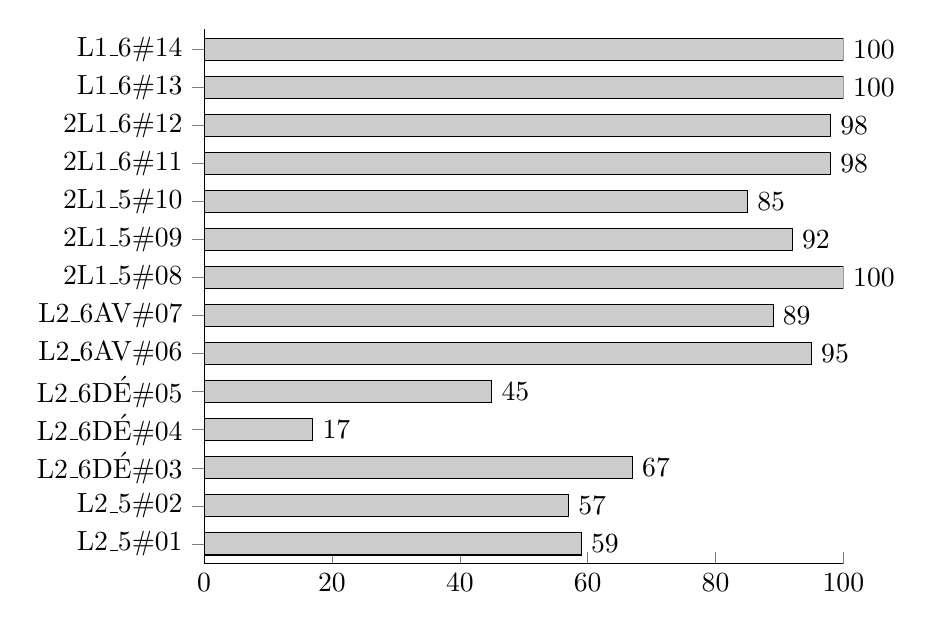
\begin{tikzpicture}
\begin{axis}[
    xbar,
    axis lines* = left,
    xmin = 0,
    xmax = 100,
    ytick = {1,2,3,...,14},
    yticklabels = {L2\_5\#01,
    L2\_5\#02,
    L2\_6DÉ\#03,
    L2\_6DÉ\#04,
    L2\_6DÉ\#05,
    L2\_6AV\#06,
    L2\_6AV\#07,
    2L1\_5\#08,
    2L1\_5\#09,
    2L1\_5\#10,
    2L1\_6\#11,
    2L1\_6\#12,
    L1\_6\#13,
    L1\_6\#14
    },
    nodes near coords,
    nodes near coords style={font=\normalsize,black},
    nodes near coords align={horizontal},
    width = .8\textwidth,
    bar width = 8pt,
    enlarge y limits = .04,
    ]
    \addplot+[draw=black,fill=black!20]
    coordinates {
    (59,1)
    (57,2)
    (67,3)
    (17,4)
    (45,5)
    (95,6)
    (89,7)
    (100,8)
    (92,9)
    (85,10)
    (98,11)
    (98,12)
    (100,13)
    (100,14)
    };
\end{axis}
\end{tikzpicture}
\caption{\label{fig:kihlstedt:2} Pourcentages des contextes du passé marqués au passé (\citealt[24]{GranfeldtEtAl2007}). Légende : L1 = Groupe de contrôle ; 2L1 = Groupe des bilingues simultanés ; L2 = Groupe des bilingues successifs ; AV = niveau de compétence avancée ; DÉ = niveau de compétence débutante ; le chiffre suivant le trait bas (i.e., \_5 ou \_6) indique l’âge de l’enfant au moment du recueil de données ; le symbole \textit{\#} précède le numéro attribué à chaque participant.}
\end{figure}

Reste cependant à déterminer ce que recouvrent exactement les chiffres de la \figref{fig:kihlstedt:2} et, plus précisément, les fonctions des emplois du passé chez les deux enfants eL2 dont les scores étaient le plus rapprochés à ceux repérés chez les enfants 2L1. Ainsi, les productions des deux enfants eL2 ayant les scores les plus élevés au marquage du passé à l’âge de 6 ans -- c’est-à-dire, au début de l’enquête -- ont été choisies pour la présente étude du développement morphologique (cf. Tableau~\ref{tab:kihlstedt:1}).


\begin{table}
\begin{tabularx}{\textwidth}{Qllllll}
\lsptoprule
Groupe & \multicolumn{2}{c}{L1} & \multicolumn{2}{c}{ 2L1} & \multicolumn{2}{c}{eL2}\\
\midrule
Prénom\footnote{Les prénoms sont des pseudonymes afin de veiller à l’anonymat des enfants.} & Anneli & Anna & Elvis & Lina & Lena & Nancy\\
Age & 7;0 & 5;5 & 6;11 & 6;5 & 7;1 & 6;7\\
\textit{Age-of-Onset}  (français) & \multicolumn{2}{c}{Naissance} & \multicolumn{2}{c}{Naissance} & 3;6 & 3;4\\
\lspbottomrule
\end{tabularx}
\caption{Choix des enfants\label{tab:kihlstedt:1}}
\end{table}

\subsection{La morphologie temporelle dans une expérience de production induite}\label{sec:kihlstedt:4.4}\largerpage

Un test ludique de complètement des phrases a été soumis aux quatre enfants bilingues 2L1 et eL2 (i.e., Elvis, Lina, Lena et Nancy) et à deux autres enfants monolingues (i.e., Eric et Louis\footnote{Les deux enfants L1 du \tabref{tab:kihlstedt:1} (i.e., Anna et Anneli) n’ont pas pu faire ce test, car elles n’étaient pas âgées d’entre 8 et 9 ans au moment du prélèvement. Dans cette tâche, l’âge était le même pour tous les enfants, et le développement longitudinal n’était pas au centre de l’intérêt.}). Au moment du test, tous les élèves étaient âgés de 8 à 9 ans. Cette expérience repose sur une tâche qui consiste à compléter des énoncés avec un temps verbal attendu. Pour éliciter les temps du \textit{passé composé} (PC) et de \textit{l’imparfait} (IMP), on a présenté aux enfants une série de dix petites histoires sur un écran d’ordinateur. Chaque histoire était composée de quatre images représentant une action à différents moments de la vie d’un personnage ou d’un animal. La procédure utilisée était la suivante : tout d’abord, le personnage et le contexte étaient présentés à l’enfant~$-$ par exemple : \textit{Ce petit chien adore mordre tout ce qu’il trouve parce que comme ça il se fait les dents […]}. Puis on a introduit une séquence de quatre images (une à la fois). Chaque image représentait un événement évoquant le même verbe, par exemple \textit{mordre.} Les commentaires de l’expérimentateur, lors de la présentation de chaque image, permettaient de situer l’événement dans le temps (présent, futur, passé). L’enfant devait ensuite compléter la dernière proposition énoncée par l’expérimentateur, qui contenait des expressions adverbiales contraignantes, telles que \textit{maintenant} (pour le présent), \textit{hier matin/soir/après-midi} (pour le passé composé), \textit{il y a longtemps, encore petit, souvent} (pour l’imparfait), ou \textit{plus tard, dans quelques années} (pour le futur simple). L’expérimentateur, toujours l’institutrice de l’enfant, a introduit les expressions adverbiales selon des consignes très précises : il ne fallait à aucun moment mentionner le verbe de l’événement. Dans ce qui suit, nous donnons un exemple d’une séquence d’images, des consignes et des réponses attendues pour le verbe \textit{mordre}~concernant l’imparfait et le passé composé :


\begin{quote}
«~Voici un petit chien. Ce petit chien adore mordre tout ce qu’il trouve parce que comme ça il se fait les dents. Il cherche de quoi mordre maintenant : une chaussure, un os, un bout de bois…Donc maintenant on va raconter l’histoire ensemble, je commence et tu continues~»


\textbf{Image} \textbf{2} \textbf{:} Tu vois ce petit os ici (pointant l’image). Le chien se rappelle qu’il y a très longtemps, encore   petit, tous les jours… \textbf{?~}(voix montante, se tournant vers l’enfant)



\textbf{Réponse} \textbf{visée} : il mordait un petit os (IMP).



\textbf{Image} \textbf{3} \textbf{:} Il se rappelle aussi que hier matin, en jouant avec le chat\textbf{…} ? (pointant l’image)…



\textbf{Réponse} \textbf{visée} : il a mordu la queue du chat (PC).
\end{quote}


Au total, dix verbes ont été testés~pour ces deux temps verbaux: \textit{boire, cueillir, conduire, écrire, lire, manger, mettre, mordre, peindre, réparer}. 


\section{Résultats}\label{sec:kihlstedt:5}
\subsection{Développement des temps verbaux du passé}\label{sec:kihlstedt:5.1}\largerpage

Si l’on tient compte des toutes les formes du passé de nos jeunes apprenantes eL2, on peut constater une évolution similaire chez Lena et Nancy entre le premier enregistrement (Lena avait tout juste 7 ans) et le deuxième enregistrement (cf. Tableau~\ref{tab:kihlstedt:2}, groupe eL2). Cette tendance s’illustre par une augmentation de 43 à 60 des formes au PC et de 79 à 115 formes à l’IMP, chez Lena ; et par une augmentation de 17 à 27 au PC et de 2 à 41 formes à l’IMP, chez Nancy. Dans les deux autres groupes, la variabilité individuelle est plus importante et la relation entre la première passation et la deuxième est plus aléatoire : chez les 2L1, il y a une augmentation chez Elvis, mais pas chez Lina. La même remarque vaut pour les deux enfants L1. La diversification lexicale de \textit{l’imparfait} se développe de manière plus nette chez les enfants eL2 que chez les autres enfants, alors que le \textit{passé composé} est utilisé avec toutes sortes de verbes chez tous les enfants dès le début de l’enquête. On en déduit que cette forme -- en augmentation chez Lena et Nancy si l’on compare leur premier et deuxième enregistrement -- est quasiment acquise chez tous les enfants, ce qui est conforme à la littérature : \textit{le passé composé} est acquis avant \textit{l’imparfait} chez des adultes L2 et des enfants L1 et 2L1 (cf. \sectref{sec:kihlstedt:2.2}).


\begin{sidewaystable}

\begin{tabularx}{\textwidth}{Qrrrrrrrrrrrr}

\lsptoprule

 & \multicolumn{4}{c}{Groupe eL2} & \multicolumn{4}{c}{Groupe 2L1} & \multicolumn{4}{c}{Groupe L1}\\
 \midrule
Participants & \multicolumn{2}{c}{Lena} & \multicolumn{2}{c}{Nancy} & \multicolumn{2}{c}{Lina} & \multicolumn{2}{c}{Elvis} & \multicolumn{2}{c}{Anneli} & \multicolumn{2}{c}{Anna}\\
Age & 7;1 & 9;1 & 6;7 & 8;7 & 6;5 & 8;3 & 6;11 & 8;7 & 7;0 & 7;11 & 5;5 & 6;3\\
Exposition & 3 ans & 5 ans & 3 ans & 5 ans & \multicolumn{4}{c}{Depuis naissance} & \multicolumn{4}{c}{Depuis naissance}\\
PC & 43 & 60 & 17 & 27 & 21 & 21 & 10 & 19 & 8 & 26 & 14 & 11\\
IMP & 79 & 115 & 2 & 41 & 13 & 14 & 3 & 16 & 3 & 18 & 17 & 6\\
PQP & 0 & 1 & 0 & 0 & 0 & 4 & 0 & 0 & 2 & 5 & 1 & 3\\
IMP parmi formes au passé & 65\% & 65\% & 10\% & 60\% & 23\% & 35\% & 23\% & 45\% & 23\% & 36\% & 51\% & 30\%\\
dont verbes dynamiques & 0\% & 29\% & 0\% & 25\% & 61\% & 50\% & 12\% & 43\% & 33\% & 25\% & 18\% & 0\%\\
\lspbottomrule
\end{tabularx}

\caption{Distribution des formes du passé par groupes\protect\footnote{Légende : PC = passé composé, IMP = imparfait, PQP = plus-que-parfait.}}
\label{tab:kihlstedt:2}
\end{sidewaystable}


Les résultats montrés au Tableau 2 suggèrent les indices développementaux qui suivent :


\begin{itemize}
\item 
Les chiffres similaires entre les trois groupes d’enfants, et notamment entre 2L1 et eL2, mis en évidence dans la \figref{fig:kihlstedt:2}, recouvrent des réalisations et des distributions différentes des formes du passé, avec un développement plus marqué en eL2 qu’en 2L1 ou L1.

\item 
Les deux apprenantes eL2 augmentent le nombre des formes du passé à 8 ans par rapport à 6~ans.

\item\sloppy
Nancy augmente considérablement son emploi de \textit{l’imparfait} entre les deux enregistrements. En cela, elle se rapproche de ce que font les adultes, chez qui l’\textit{imparfait}, quand il émerge, apparaît en quantités plus faibles que le \textit{passé composé.} Lena utilisait déjà beaucoup de formes à \textit{l’imparfait} à la première passation, mais presque exclusivement reliées à la troisième personne du singulier du verbe \textit{être} (i.e. \textit{était}). Elle était probablement à un stade plus avancé que Nancy à 6 ans.

\item 
L’augmentation des formes à l’\textit{imparfait} est accompagnée d’une hausse remarquable des verbes dynamiques chez les deux apprenantes eL2 entre 6 et 8 ans (de 0 à 29\% et de 0 à 25\%, respectivement). Il y a donc une diversification lexicale des formes à \textit{l’imparfait,} au-delà des occurrences initiales des verbes d’état qui s’opère entre 6 et 8 ans.

\item 
Les bilingues simultanés utilisent des verbes dynamiques dès 6 ans, tout comme les enfants monolingues. Par ailleurs, la variation interindividuelle est globalement plus importante chez les deux filles monolingues et les deux enfants 2L1, ce qui pourrait impliquer que leur maîtrise morphologique est plus avancée ou achevée depuis un certain temps. Dans le cas d’Elvis, on constate une courbe montante des formes du passé, notamment dans le nombre d’occurrences et les proportions de l’\textit{imparfait.} Cependant, à la différence des enfants eL2, il utilise déjà des verbes dynamiques à \textit{l’imparfait} à 6 ans.

\end{itemize}

\begin{sloppypar}
On assiste donc à un certain retard des enfants eL2 par rapport aux autres groupes enfantins, notamment concernant le développement lexical de \textit{l’imparfait.} Selon \citet{Kihlstedt2002}, l’émergence des verbes dynamiques à l’i\textit{mparfait} constitue un trait important pour discriminer entre différents stades avancés d’acquisition en adulte L2 (voir \textit{supra} \sectref{sec:kihlstedt:1.2.2} et \sectref{sec:kihlstedt:2.2}). Certains apprenants adultes restent longtemps sur le stade des verbes d’état. Il semble en être autrement chez les enfants eL2, qui utilisent des verbes dynamiques à \textit{l’imparfait} dans des proportions élevées à 8 ans. Plus précisément, dès que Lena et Nancy augmentent le nombre d’occurrences de cette forme, la variation lexicale suit, au-delà des verbes d’état (voir les chiffres des eL2 à la deuxième passation, Tableau 2). Pour illustrer ces emplois, voici quelques exemples. Dans \REF{ex:kihlstedt:1} et \REF{ex:kihlstedt:2}, une question ancrée à \textit{l’imparfait} déclenche des séries de verbes dynamiques différents~chez les deux enfants :
\end{sloppypar}

\ea%1
    \label{ex:kihlstedt:1}
    INT\footnote{Légende de transcription : INT = interlocuteur, ici l’institutrice ; \# = reprise ou reformulation ; / = pause.}: Tiens l’été dernier qu’est-ce que tu faisais le matin toujours ?



    NANCY:  Je me \textbf{\textit{réveillais}}.



    INT:  Mhm.



    NANCY:  Et je me \textbf{\textit{brossais}} les dents. 



    INT:  Mhm . Et le soir alors qu’est-ce que tu faisais en plus ?



    NANCY: \#\# Mm \#\# je \textbf{\textit{lisais}} un livre qui était comme ça.



    INT:  Gros comme ça dis donc.



    NANCY:  Et \#\# on \textbf{\textit{avait}} pas toujours le droit mais on \textbf{\textit{mangeait}} efterrätt (= le dessert). \hfill[Nancy, deuxième passation]
\z


\ea\label{ex:kihlstedt:2}  
INT:  Alors qu’est-ce que tu avais l'habitude de faire le matin ?



  LENA: Me baigner hehe. [//] Je me \textbf{\textit{baignais} }toutes \# les jours\textbf{ . }[…] et \# aussi je \textbf{\textit{prenais}} des poissons avec un filet. \hfill[Lena, deuxième passation]
\z


Cette variation lexicale est accompagnée d’une diversité fonctionnelle ; les deux informantes utilisent~fréquemment \textit{l’imparfait} d’habitude -- comme dans \REF{ex:kihlstedt:1} et \REF{ex:kihlstedt:2} -- et aussi \textit{l’imparfait} d’incidence -- exemples \REF{ex:kihlstedt:3} et \REF{ex:kihlstedt:4} -- sans que l’une des valeurs semble présenter plus de problèmes que l’autre. Parfois la valeur d’incidence émerge même sans sollicitation de la part de l’adulte \REF{ex:kihlstedt:4}~  :



\ea%3
    \label{ex:kihlstedt:3}
    INT:  Alors qu’est-ce que vous étiez en train de faire dans la classe quand j’étais de l’autre côté?



    Nancy:  On \textbf{\textit{parlait}}. \hfill[Nancy, deuxième passation]
\z


\ea \label{ex:kihlstedt:4}   Lena:  Et il y \textbf{\textit{avait}}  un chose \# de pierre et un trou dans ce pierre .



    INT:  Au plafond de la grotte ?



  Lena:  Oui et au-dessus du bassin il \textbf{\textit{tombait}} de l'eau vert qui \textbf{\textit{était}} comme le ketchup vert qui \textbf{\textit{tombait}} dans le bassin. et le bassin c’\textbf{\textit{était}} vert de [?] ketchup. J\textbf{\textit{’ai} \textit{tombé}} dans le ketchup vert. 
  
  \hfill[Lena, deuxième passation]
\z


Ce dernier exemple est intéressant à plusieurs titres : il contient un verbe télique de caractère ponctuel à \textit{l’imparfait,} ce qui est un usage marqué et peu fréquent même en français natif~(voir \citealt{IzquierdoKihlstedt2019}). De plus, le verbe \textit{tomber} est utilisé ici tantôt à \textit{l’imparfait,} tantôt au \textit{passé composé} -- avec un auxiliaire erroné -- pour reprendre la trame narrative. Tout indique que Lena a découvert l’aspectualisation morphologique en français et s’en sert à son gré, parfois en faisant varier le même verbe lexical. Ce type d’emploi n’est jamais, ou très rarement, attesté dans nos études sur des adultes suédophones (\citealt{Kihlstedt2002, Kihlstedt2009, Kihlstedt2015}).



En résumé, on assiste, chez les deux enfants eL2 observés, à un développement dans l’emploi des formes du passé, notamment \textit{l’imparfait,} pendant les deux années de durée de l’étude. Ce développement se reflète moins en termes de fréquences que de diversification fonctionnelle : les relations complexes d’habitualité et de progressivité sont attestées dès le deuxième entretien, alors qu’elles sont absentes dans le premier entretien, contrairement aux deux autres groupes.


\subsection{La morphologie temporelle dans une tâche de production contrôlée}\label{sec:kihlstedt:5.2}

Cette étude met au premier plan la question de savoir si les enfants, surtout les eL2, ont généralisé les règles concernant la morphologie aspecto-temporelle à 8 ans. Deux observations générales ressortent. Premièrement, la rareté de certaines formes sollicitées en français oral pourrait expliquer une stratégie observée chez tous les groupes d’enfants, que l’on pourrait appeler la stratégie «~analytique~».\footnote{Le procédé consistant à séparer l’information morphologique et lexicale en deux formes, appelé \textit{stratégie analytique,} a été massivement attesté et discuté chez des adultes acquérant le français en milieu naturel du projet ESF (\citealt{BenazzoStarren2007, Véronique2009}). Il pourrait s’agir d’un phénomène universel, qui dépasse la distinction apprenant enfant / apprenant adulte (pour une discussion, voir \citealt{KihlstedtSchlyter2009}).} Il s’agit des cas où les enfants prennent appui sur un verbe modal pour produire la forme morphologique visée, donnant ensuite l’information lexicale de l’événement à l’infinitif : \textit{pouvait boire} (groupe 2L1), \textit{pouvait cueillir} (groupe L1), ou \textit{pouvait prendre} (\textit{prendre} renvoyant à \textit{cueillir}) chez Nancy -- groupe L2 -- à la place de \textit{buvait} et \textit{cueillait}. 



Comme il en ressort de la \figref{fig:kihlstedt:3}, qui résume les données de la tâche de production contrôlée, tous les enfants ont produit à peu près le même niveau de réponses attendues pour \textit{le passé composé}. La deuxième observation -- la plus importante -- concerne le clivage observé entre les enfants 2L1 et eL2 relativement à certains temps verbaux. On constate une différence nette entre les enfants L1 et 2L1 d’une part, et les enfants eL2 de l’autre, pour \textit{l’imparfait} : on trouve ainsi seulement 45\% des réponses attendues à l’IMP chez ces derniers, ce qui  contraste avec le 100\% des L1 et des 2L1, respectivement.\footnote{Légende : PC = passé composé, IMP = imparfait, L1 = enfants monolingues, 2L1 = bilingues simultanés, L2 = bilingues successifs.}



\begin{figure}
%%\includegraphics[width=\textwidth]{figures/./ObjectReplacements/Object 3}
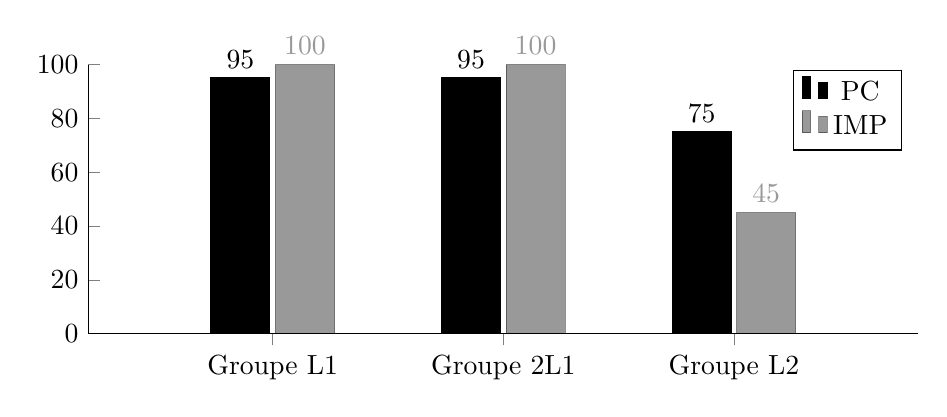
\begin{tikzpicture}
\begin{axis}[
    ybar,
    axis lines* = left,
    ymin = 0,
    ymax = 100,
    xtick = {1,2,3},
    xticklabels = {Groupe L1,Groupe 2L1,Groupe L2},
    nodes near coords,
    width = \textwidth,
    height = 5cm,
    bar width = .75cm,
    enlarge x limits = .4,
    ]
    \addplot+[black] coordinates {(1,95) (2,95) (3,75) };
    \addplot+[black, opacity = .4] coordinates {(1,100) (2,100) (3,45)};
    \legend{PC,IMP}
\end{axis}
\end{tikzpicture}
\caption{\label{fig:kihlstedt:3}Pourcentages des réponses attendues par les enfants (adapté de \citealt[103]{KihlstedtSchlyter2009})}
\end{figure}

Concernant l’IMP, les enfants L2 se comportent conformément à ce qui a été observé pour des adultes L2 : en réponse à des questions où une réponse à l’IMP est attendue, les enfants L2 utilisent soit une forme de base au présent à référence passée, soit le PC. Et ce, malgré l’aisance avec laquelle l’IMP est utilisé dans le dialogue par les mêmes enfants pour cette même tranche d’âge, comme on l’a vu dans la section précédente. Lena répond dans la moitié des cas au présent de l’indicatif quand la question porte sur l’IMP, tel qu’illustré dans l’exemple \REF{ex:kihlstedt:5}, alors que Nancy, de son côté, recourt plutôt au passé composé dans des contextes imper\-fectifs \REF{ex:kihlstedt:6} :


\ea%5
    \label{ex:kihlstedt:5}
    INT: Et pendant qu’il marche il se souvient qu’il y a très très longtemps alors beaucoup plus petit que maintenant hein?

Lena : \textbf{\textit{Il} \textbf{peint} }des petits voitures en rouge.

INT: Oui il peignait de petites voitures en rouge. 

\hfill[Lena, deuxième passation]
\z

\ea%6
    \label{ex:kihlstedt:6}
 INT : et il se souvient qu’il y a très longtemps, encore bébé….  

  Nancy : qu’il \textbf{a} \textbf{bu} dans un biberon.

  INT : oui qu’il buvait dans un grand bibéron. 
  
  \hfill[Nancy, deuxième passation]
\z


Il est intéressant de noter que dans les deux exemples précédents, l’institutrice reformule la réponse des enfants à la forme visée : \textit{peignait} \REF{ex:kihlstedt:5}, \textit{buvait} \REF{ex:kihlstedt:6}. Or, cela n’a pas d’effet sur les réponses ultérieures à l’imparfait. Il se manifeste une certaine «~surdité~» à l’usage de l’imparfait avec des verbes autres que des verbes d’état chez les deux enfants eL2. Les résultats concernant les enfants bilingues successifs sont d’autant plus étonnants que les deux informantes arrivent, au même moment, à utiliser librement des séquences des formes qui semblent ici difficiles~dans la conversation, ce qui ressort des exemples \REF{ex:kihlstedt:1} à \REF{ex:kihlstedt:4} \textit{supra}. Il semblerait donc que la tâche ait un impact sur la performance de Lena et de Nancy, impact non observé chez leurs camarades monolingues et bilingues simultanés, où la morphologie imperfective est utilisée correctement et généreusement aussi bien dans le test que dans la conversation.


\section{Discussion}\label{sec:kihlstedt:6}

\subsection{Des études des cas}\label{sec:kihlstedt:6.1}

Les résultats présentés \textit{supra} portent sur un nombre très limité d’enfants ; ne permettant pas de généralisations au-delà de ce petit échantillon. Cependant des études de cas d’enfants suivis longitudinalement telle que la présente réunissent certains avantages. Premièrement, elles fournissent une image holistique mais détaillée du développement linguistique des enfants (\citealt{LindqvistBardel2014, VallerossaBardelàparaître}). Cela est d’autant plus important que, de manière générale, les différents types de bilinguisme présentent en eux-mêmes des problématiques spécifiques, donnant lieu à de grandes variations. Deuxièmement, elles constituent un outil précieux pour le test d’hypothèses et l’élaboration ultérieure de théories \citep{Hammarberg2022}, qui pourront par la suite être testées sur des populations plus importantes. 


\subsection{Le bilinguisme successif : semblable ou différent du bilinguisme simultané ?}\label{sec:kihlstedt:6.2}

Dans ce qui précède, il a été constaté que les bilingues successifs, avec un début d’acquisition du français entre 3 et 4 ans, se comportent tantôt comme des adultes, tantôt comme des enfants bilingues simultanés. A 6 ans, les bilingues successifs marquent le passé dans des contextes obligatoires dans la même mesure que les bilingues simultanés. Le développement à 8 ans se caractérise par un emploi plus riche et diversifié des formes et des fonctions des formes du passé, et notamment une émergence des formes à \textit{l’imparfait} avec toutes sortes de verbes. Cette progression est déjà en place à 6 ans chez les bilingues simultanés et les monolingues. Ainsi, concernant le développement, il semblerait que les eL2 ressemblent aux enfants L1 et 2L1, quoiqu’avec en certain retard (différence de \textit{rate}). Or, même si le développement morphologique en français est un peu plus lent en eL2, l’utilisation \textit{discursive} et l’aspectualisation morphologique que permet le français mais pas le suédois, qui ne marque pas l’aspect, semblent suivre des paliers communs aux trois modes d’acquisition enfantine. En revanche, les enfants eL2 se différencient des 2L1 dans une tâche dirigée de production induite, où leur comportement ressemble plutôt à celui des adultes (différence de \textit{route}), ce qui a été observé pour l’usage de formes idiosyncrasiques et de réponses inadéquates dans des contextes censés induire des formes à \textit{l’imparfait}.


\subsection{Tentatives d’explication}\label{sec:kihlstedt:6.3}

Les enfants L2 ont donc encore, à 8--9 ans et après 4 ans d’exposition au français en immersion scolaire, quelques traces d’une acquisition différente de leurs camarades L1 et 2L1. Qu’impliquent ces résultats pour notre questionnement général sur les différents modes d’acquisition ?  Faut-il les interpréter comme une preuve d’une différence fondamentale, tout au moins partielle, entre bilingues simultanés et successifs ? Et si une telle différence existe, où convient-il de situer le seuil crucial (en anglais, \textit{cut-off point}) à partir duquel l’acquisition est plus de nature «~eL2~» que «~2L1~» ? Y a-t-il un ou plusieurs seuils cruciaux ? Ou ne s’agit-il pas du tout d’un âge crucial mais juste de la complexité de la tâche ? Les différences observées entre 2L1 et eL2, vont-elles s’estomper avec le temps ? 



La différence de tâche joue certainement un rôle. Dans la conversation libre, les mêmes enfants eL2 ont donné libre cours à ce qu’elles souhaitaient exprimer en réponse à des questions sur le passé et ont montré une maîtrise prononcée de la sémantique complexe de \textit{l’imparfait} et de l’opposition \textit{passé composé} / \textit{imparfait}. Les réalisations induites de \textit{l’imparfait} se font plus difficilement dans une tâche contraignante que dans les productions spontanées. Mais la tâche n’explique pas toute la difficulté de nos jeunes apprenantes. Nous pensons qu’il faudrait aussi tenir compte de la différence entre deux types de capacités morphologiques : celle qui est liée à la réalisation «~matérielle~» ou à l’instanciation des formes au niveau structurel, et celle qui consiste à pouvoir utiliser la morphologie temporelle d’une manière sémantiquement et fonctionnellement adéquate, dans tout type de contexte. Les données ici présentées confirment que les bilingues simultanés ont bien les deux capacités, mais les bilingues successifs pas encore. 

On peut ainsi entrevoir un caractère spécifique des enfants bilingues successifs. En particulier, il semble que la polyfonctionnalité de \textit{l’imparfait} est effectivement plus facile à maîtriser pour eux que pour d’autres apprenants L2 du français. \citet{Ayoun2004}, dans ses études sur des apprenants anglophones adultes de français, fait valoir que les apprenants progressent dans leur emploi du \textit{passé composé,} mais pas dans celui de \textit{l’imparfait,} à cause de la complexité sémantique de ce dernier. La plus grande différence entre adultes et enfants qui acquièrent une L2 réside dans le fait que le développement cognitif est abouti chez l’adulte, alors qu’il est toujours en cours chez l’enfant. On peut supposer que les enfants eL2, de ce fait, profitent d’une plus grande malléabilité cognitive qui les dispose davantage à atteindre la maîtrise de la subtilité des fonctions de \textit{l’imparfait} en L2, souvent considérées comme «~les derniers bastions~» dans l’acquisition du français. Cette explication semble cohérente avec l'idée ci-dessous [c’est nous qui soulignons en gras le segment pertinent à notre propos] : 


\begin{quote}
In brief, each native language has trained its speakers to pay different kinds of attention to events and experiences when talking about them. \textbf{This training is carried out in childhood and is exceptionally resistant} in adult second language acquisiton.\hbox{}\hfill\hbox{(\citealt[23]{Slobin1996})}
\end{quote}


Les suédophones acquérant le français pendant leur enfance auraient développé, «~par entrainement~», une conceptualisation particulière dans leur façon de raconter des événements,~en prêtant attention à certains aspects des événements plutôt qu’à d’autres. Il s’agit, selon Slobin, d’une empreinte indélébile, qui est exceptionnellement résistante à être restructurée en L2. La L1 de ces bilingues précoces, le suédois, ne grammaticalise pas la distinction perfectif / imperfectif. Si l’acquisition du français L2 ne commence pas suffisamment tôt, à savoir pendant que le développement cognitif fondamental se poursuit encore, il serait plus difficile d’acquérir la distinction aspectuelle du français, alors que les enfants eL2 étudiés ici ressemblent plus aux enfants 2L1 à cet égard.



D’un autre côté, les eL2 et les 2L1 se différencient dans la deuxième partie de nos résultats. Une explication possible serait que le développement morphologique initial et le développement de la morphologie dans les discours – par exemple, dans des récits – prennent tôt des itinéraires (des \textit{routes}) d’acquisition différents pour les bilingues successifs. Les 2L1 acquièrent et séparent dès le début deux systèmes morphologiques. Ces systèmes sont ancrés de façon stable et prêts à être mobilisés dans toutes sortes de tâches, même complexes, comme celle de l’expérience de production induite décrite ci-dessus. Les L2 ont développé un seul système morphologique, celui du suédois, pendant leurs premières années de vie (jusqu’à 4 ans), et ont plus de problèmes, à 8 ans, pour faire ce que les L1 et les 2L1 arrivent à faire dans une tâche contrôlée, cognitivement plus complexe que la conversation libre. Nos résultats préliminaires conféreraient ainsi une spécificité aux enfants eL2, dont le développement morphologique ne serait ni tout à fait comme celui des bilingues simultanés, ni tout à fait comme celui des adultes L2.



\section{Conclusion}\label{sec:kilhstedt:7}


Dans ce qui précède, nous avons comparé le développement du temps et de l’aspect en français chez quelques enfants en âge scolaire, issus du bilinguisme successif et simultané. L’approche qualitative nous a permis de montrer que l’utilisation spontanée des temps verbaux du passé suivrait des étapes communes, avec un léger retard des enfants eL2, alors que dans des tests plus ciblés, les bilingues successifs se différencient clairement des deux autres groupes d’enfants (i.e., 2L1 et L1). Il a été proposé que l’enfant eL2 constitue un cas particulier d’acquisition L2, qui mériterait plus d’attention dans les études ultérieures. Les deux enfants eL2 de la~présente étude ont commencé l’acquisition du français à 3 ans et demi et à 4 ans. Est-ce qu’une exposition continue et durable à la L2 à partir d’un âge plus tardif aurait le même résultat ? Quel est le poids relatif de l’AOA (\textit{age of onset)} chez des enfants issus du bilinguisme successif par rapport (a) à la durée et à la qualité de l’exposition~(immersion partielle restreinte à l’établissement scolaire ou totale, sensibilisation explicite à la distinction perfectif / imperfectif), et (b) aux aspects du phénomène étudié (conversations libres ou expérience ciblée)? Des études ultérieures, avec d’autres combinaisons de langues et des populations plus importantes permettraient d’apporter des éléments de réponse plus poussés sur le statut particulier de l’enfant eL2. 

\section*{Remerciements}
Daniel Véronique a toujours été, depuis notre première rencontre à Eurosla à Aix-en-Provence en 1994, un modèle pour affiner ma réflexion sur la RAL (Recherche en Acquisition des Langues, acronyme qui vient de lui). Sa conception du modèle de la grammaticalisation pour les langues secondes/étrangères (particulièrement pour la temporalité en adulte L2), ses grandes connaissances de la littérature acquisitionnelle anglo-saxonne, ses multiples travaux sur l’application des résultats en RAL aux divers contextes d’enseignement en France, ainsi que son remarquable esprit de synthèse ont été, à travers les années, une grande source d’inspiration.

\sloppy\printbibliography[heading=subbibliography,notkeyword=this]
\end{otherlanguage}
\end{document} 
